%!TEX root = Problems2_main.tex

\makeatletter
\renewcommand{\@maketitle}{
\newpage
 \null
 \vskip 2em%
 \begin{center}%
  {\Large \@title \par}%
 \end{center}%
 \par} \makeatother

\begin{center}
\Huge University Physics Problems 2\\[1em]
\large March 2013
\end{center}

\section{Reflecting}
	Two periscopes are constructed as shown below. In each case, the periscope is used to observe a person with the word BEN written on their t-shirt. In each case, the light is reflected from mirror 1 to mirror 2 and then to the observer. For each design, what is the orientation of the word as viewed by the observer?
	\begin{figure}[ht]
	  \centering
	  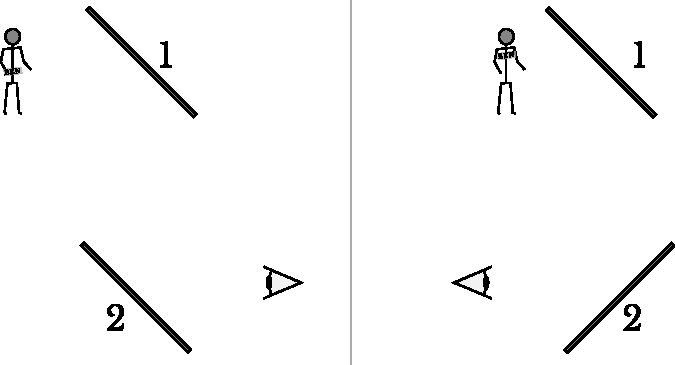
\includegraphics[width=0.6\textwidth]{periscopes.pdf}
	\end{figure}

\section{Recombining}
	A narrow beam of white light passes through a glass prism. The light is dispersed into its constituent colours. Can these rays be recombined into white light by passing them through a second prism?

\section{Throwing}
	\subsection{}
		\begin{wrapfigure}{r}{0.4\textwidth}
		  \vspace{-20pt}
		  \begin{center}
		  	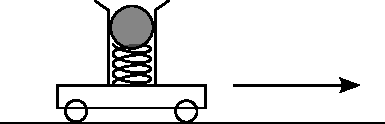
\includegraphics[width=0.35\textwidth]{trolley1.pdf}
		  \end{center}
		  \vspace{-20pt}
		\end{wrapfigure}
		A trolley rolls without friction along a track. When the trolley passes over some point in the track, the ball is released and is ejected upwards. Does it fall 
		\begin{enumerate}[label=\alph*)]
			\item in front of the tube,
			\item behind the true,
			\item back into the tube?
		\end{enumerate}

	\subsection{}
		\begin{wrapfigure}{r}{0.4\textwidth}
		  \vspace{-20pt}
		  \begin{center}
		  	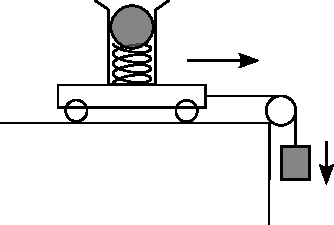
\includegraphics[width=0.35\textwidth]{trolley2.pdf}
		  \end{center}
		  \vspace{-20pt}
		\end{wrapfigure}
		The trolley is now connected via a light string and a pulley wheel to a weight and the experiment repeated. Does the ball fall
		\begin{enumerate}[label=\alph*)]
			\item in front of the tube,
			\item behind the tube,
			\item back into the tube?
		\end{enumerate}

	\subsection{}
		\begin{wrapfigure}{r}{0.4\textwidth}
		  \vspace{-20pt}
		  \begin{center}
		  	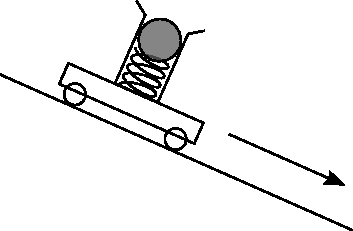
\includegraphics[width=0.35\textwidth]{trolley3.pdf}
		  \end{center}
		  \vspace{-20pt}
		\end{wrapfigure}
		The trolley is now connected via a light string and a pulley wheel to a weight and the experiment repeated. Does the ball fall
		\begin{enumerate}[label=\alph*)]
			\item infront of the tube,
			\item behind the trube,
			\item back into the tube?
		\end{enumerate}

\section{Rolling} % (fold)
	\label{sec:rolling}
	A drum has a string wrapped around a central core. The string is pulled, in case 1, it is obvious that the drum will roll to the right. In case two, the string is wrapped in the other direction around the centre of the drum. Does the drum
	\begin{enumerate}[label=\alph*)]
		\item roll to the right,
		\item roll to the left,
		\item get confused and skid along?
	\end{enumerate}
	\begin{figure}[ht]
	  \centering
	  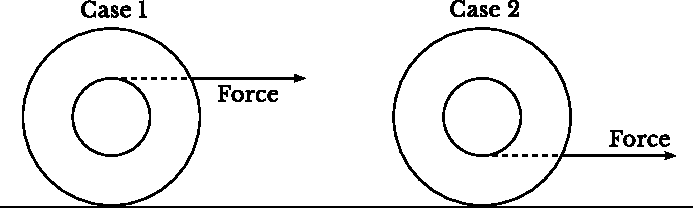
\includegraphics[width=0.7\textwidth]{drums_rolling.pdf}
	\end{figure}
% section rolling (end)

\section{Illuminating} % (fold)
	\label{sec:illuminating}
	Unpolarised light enters a single polaroid. What happens to the transmitted light? Two polaroids are now crossed at 90 degrees. What happens to the transmitted light? A third polaroid at an angle of 45 degrees is now inserted between the first two. What happens to the intensity of the light transmitted?
	\begin{figure}[ht]
	  \centering
	  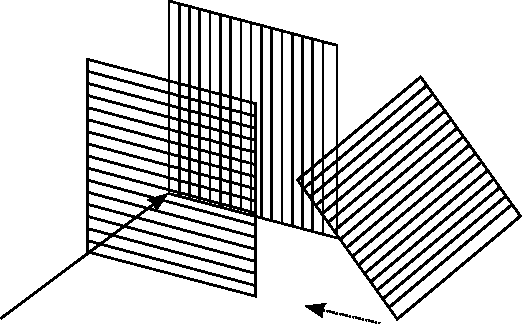
\includegraphics[width=0.4\textwidth]{polarisation.pdf}
	\end{figure}
% section illuminating (end)